%%%%%%%%%%%%%%%%%%%%%%%%%%%%%%%%%%%%% 
%% LE2I beamer template
%% Guillaume Lemaitre, October 2014
%%%%%%%%%%%%%%%%%%%%%%%%%%%%%%%%%%%%% 

\documentclass{beamer}

\usepackage[utf8]{inputenc}
\usepackage[T1]{fontenc} 
\usetheme{le2i} 

%% The amssymb package provides various useful mathematical symbols
\usepackage{amssymb}
%% The amsthm package provides extended theorem environments
\usepackage{amsthm}
%% amsmath for math environment
\usepackage{amsmath}

\DeclareMathOperator*{\argmin}{arg\,min}
\DeclareMathOperator*{\argmax}{arg\,max}
\DeclareMathOperator*{\sign}{sign}

%% figure package
\usepackage{epsf,graphicx}
\usepackage{epstopdf}
\usepackage{subfigure}
\usepackage{transparent}
\usepackage{soul}

%% In order to draw some graphs
\usepackage{tikz,xifthen}
\usepackage{tikz-qtree}
\usepackage{adjustbox}
\usetikzlibrary{decorations.pathmorphing}
\usetikzlibrary{fit}
\usetikzlibrary{backgrounds}
\usetikzlibrary{shapes,arrows,shadows}
\usetikzlibrary{calc,decorations.pathreplacing,decorations.markings,positioning}
\usetikzlibrary{snakes,decorations.text,shapes,patterns}
% \usepackage{scalefnt,lmodern,booktabs}

%% Package for cross and tick symbols
\usepackage{pifont}
\newcommand{\tick}{\color{green!60!black!80}\ding{51}}
\newcommand{\cross}{\color{red!60!black!80}\ding{55}}

\title{Centre de Calcul de l'Universit\'e de Bourgogne}
\author{Guillaume Lema\^itre \\ \texttt{guillaume.lemaitre@udg.edu}}
\date{RE-COOP \#2.2 \\ 31\textsuperscript{st} Sept. 2015}

\institute{Universit\'e de Bourgogne} 

%% Uncomment if you want to avoid thousand of bullet inside the menu
% \usepackage{etoolbox}
% \makeatletter
% \patchcmd{\slideentry}{\advance\beamer@xpos by1\relax}{}{}{}
% \def\beamer@subsectionentry#1#2#3#4#5{\advance\beamer@xpos by1\relax}%
% \makeatother

\begin{document}

% Show the title page
\begin{frame}
  \titlepage
\end{frame}

% Show the table of contents
\begin{frame}
  \tableofcontents[sectionstyle=show,subsectionstyle=show,subsubsectionstyle=hide]
\end{frame}

\section{Preface}

\subsection{Achtung!!!}

\begin{frame}
  \frametitle{Preface}
  \framesubtitle{Achtung}
  \only<1->{\begin{block}{What it will be about and will not be about ...}\footnotesize
    \begin{columns}
      \column{.2\textwidth}
        \begin{figure}
          \centering
          
\includegraphics[width=.8\textwidth]{./images/warning.png}
        \end{figure}        
      \column{.8\textwidth}
      \begin{itemize}
      \item \st{Tutorial: ``How to use the computer cluster of the UB''}
      \item ``Do we do the right thing?''
      \end{itemize}
    \end{columns}
  \end{block}}
  \only<2->{\begin{block}{Why at RE-COOP?}\footnotesize
    \begin{columns}
      \column{.2\textwidth}
      \begin{center}
        \only<2>{    
          \begin{figure}
            \centering
            
\includegraphics[width=.8\textwidth]{./images/right_person.jpg}
          \end{figure}}
        \only<3>{    
          \begin{figure}
            \centering
            
\includegraphics[width=.8\textwidth]{./images/break.jpg}
          \end{figure}}
      \end{center}
      \column{.8\textwidth}
      \begin{itemize}
      \item<2-> The right persons: PhDs and permanents 
      \item<3-> No polluted conversation in the coffee room
      \end{itemize}
    \end{columns}
  \end{block}}
\end{frame}

\subsection{What do we try to solve?}

\begin{frame}
  \frametitle{Preface}
  \framesubtitle{What do we try to solve?}
  \begin{block}{Data, data, data, ...}\footnotesize
    \begin{figure}
      \centering
      \only<1>{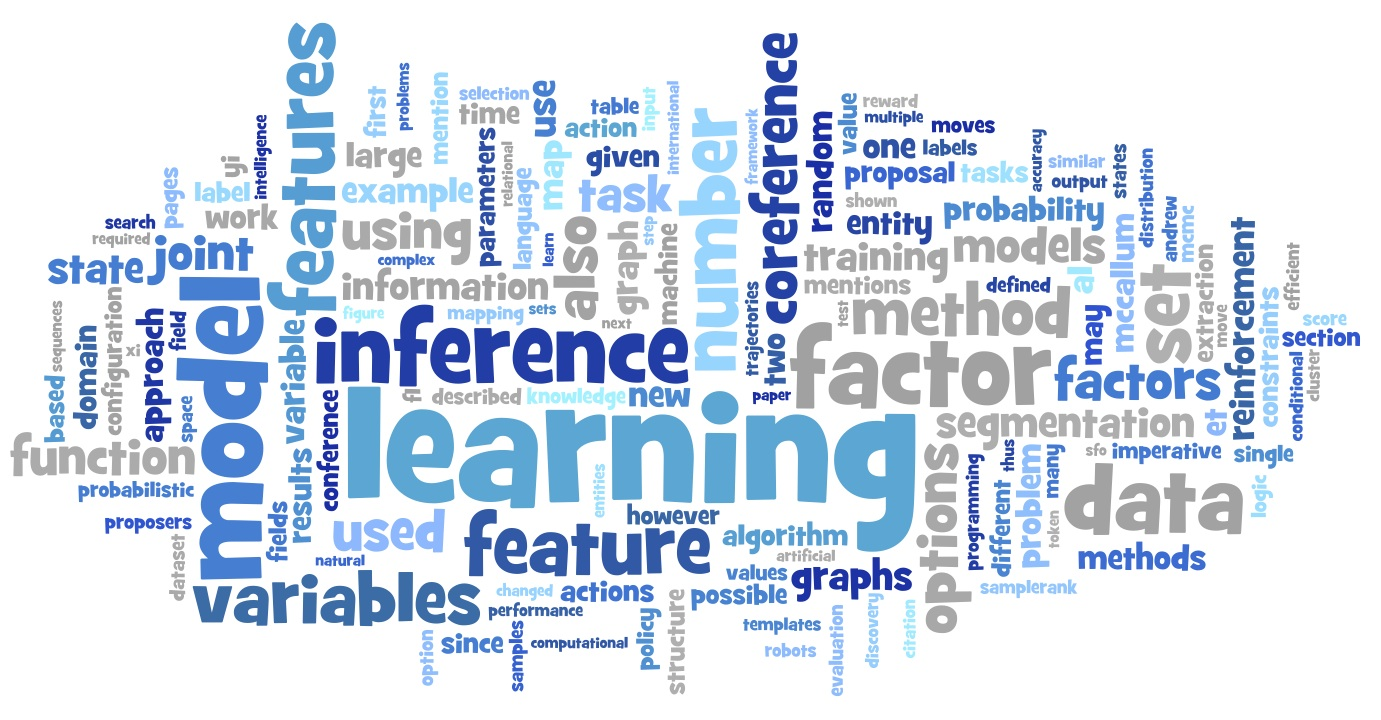
\includegraphics[width=.8\textwidth]{./images/research.jpg}}
      \only<2>{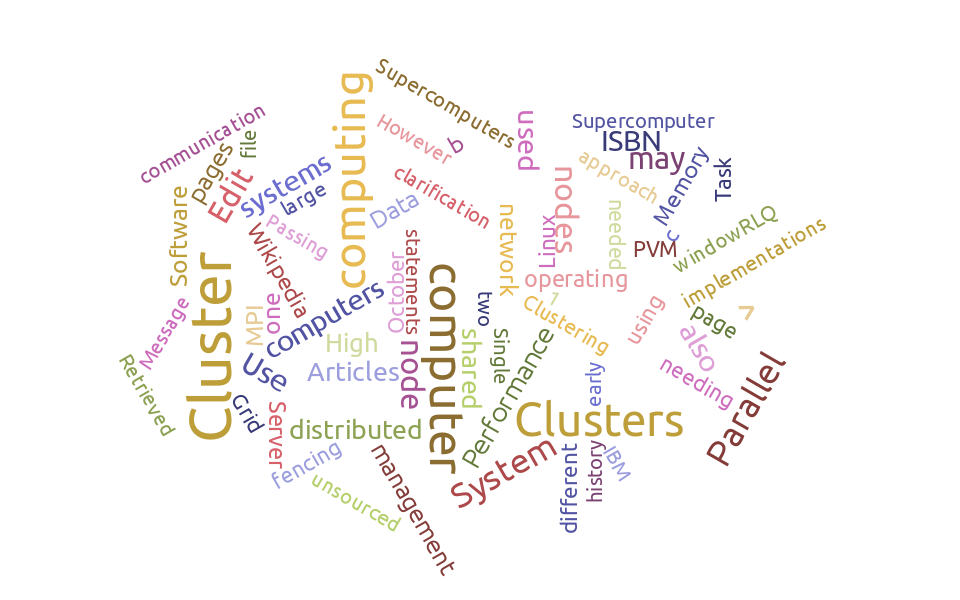
\includegraphics[width=.8\textwidth]{./images/ccub.png}}
    \end{figure}
  \end{block}
\end{frame}

\begin{frame}
  \frametitle{Preface}
  \framesubtitle{What do we try to solve?}
  \begin{block}{Some thoughts ...}\footnotesize
    \begin{itemize}
    \item<1-> Clusters do not make your research ...
    \item<2-> ... they contribute to make proper and fast research
    \item<3-> Solve problem that you could not solve before
    \item<4-> And finally save ££££\$\$\$\$
    \end{itemize}
  \end{block}
\end{frame}

\section{The CCUB}


\begin{frame}
  \frametitle{The CCUB}
  \framesubtitle{Hardware}
  \begin{block}{In numbers}\footnotesize
    \begin{itemize}
    \item \# cores: 3278 - Typically Intel Xeon 2660 at 2.0 GHz
    \item RAM: 12792 Go - Typically at least 64 Go per machine
    \item GPU: 1180 Gflops - 2 x Tesla cards
    \item HDD: 20 To per users
    \end{itemize}
  \end{block}
  \begin{block}{Organisation}\footnotesize
    \begin{itemize}
    \item Interactive computers
    \item Bash computers
    \end{itemize}
  \end{block}
\end{frame}

\begin{frame}
  \frametitle{The CCUB}
  \framesubtitle{Hardware}
  \begin{block}{Interactive computers}\footnotesize
    \begin{itemize}
    \item Large resources: up to 40 cores (80 threads) and 256 Go of RAM
    \item 3 computers to connect ``krenek''
    \item Work with usual languages: Matlab, python, C++, java, etc.
    \item Connect through SSH and possibility of Remote Desktop
    \item[\cross] Connection is time limited
    \end{itemize}
  \end{block}
  \begin{block}{Bash computers}\footnotesize
    \begin{itemize}
    \item Execution through script
    \item Deployment setting up \# cores per jobs
    \item Priority automatically set up depending of the hardware requirements and the time on the queue
    \item[\tick] Up to 7 days by executing scripts
    \end{itemize}
  \end{block}
\end{frame}

\section{Case Study}

\begin{frame}
  \frametitle{Case Study}
  \framesubtitle{Classification of SD-OCT volumes with LBP}
  \begin{block}{Background}\footnotesize
      \begin{itemize}
      \item 1 week + 1 week to design, implement, and evaluate an ML framework for DME detection
      \end{itemize}
  \end{block}
  \begin{block}{Framework}\footnotesize
      \begin{figure}
        \centering{
          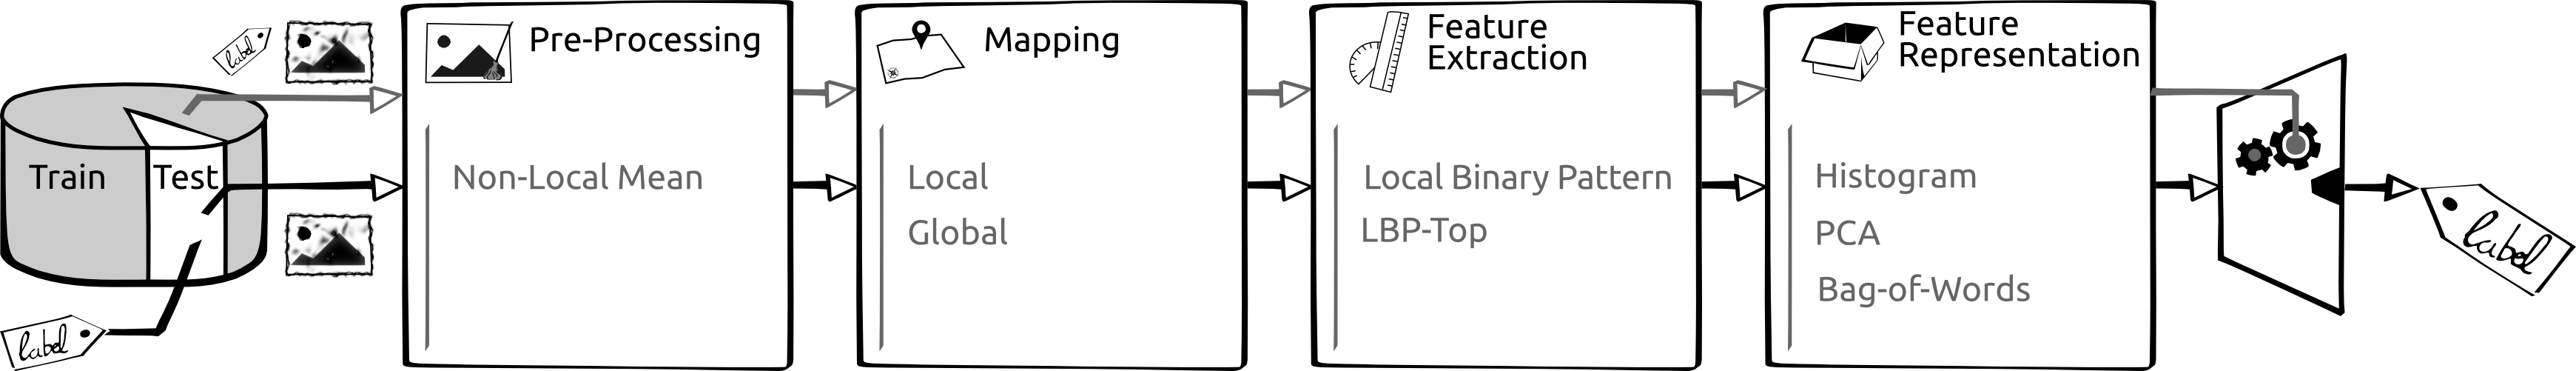
\includegraphics[width=1\textwidth]{./images/ml}}
      \end{figure}
  \end{block}
  \begin{block}{What if ...}\footnotesize
    \begin{itemize}
    \item NLM denoising $\rightarrow$ a full working day of processing
    \item Executing a script per patient $\rightarrow$ 30 jobs in parallel
    \item Harder, better, faster, stronger $\rightarrow$ parallelize in the algorithm \& patient processing
    \end{itemize}
  \end{block}
\end{frame}

\section{Requirements}

\begin{frame}
  \frametitle{Requirements}
  %\framesubtitle{Classification of SD-OCT volumes with LBP}
  \begin{block}{Spirit}\footnotesize
      \begin{itemize}
      \item The 2W: Will \& Wishes
      \end{itemize}
  \end{block}
  \begin{block}{Skill}\footnotesize
      \begin{itemize}
      \item Learn \& understand to parallelize on CPU and GPU
      \item Come back to the source - terminal/editor/compiler
      \item Move to linux
      \end{itemize}
  \end{block}
\end{frame}

\begin{frame}
  \frametitle{Requirements}
  %\framesubtitle{Classification of SD-OCT volumes with LBP}
  \begin{figure}
    \centering{
      \only<1>{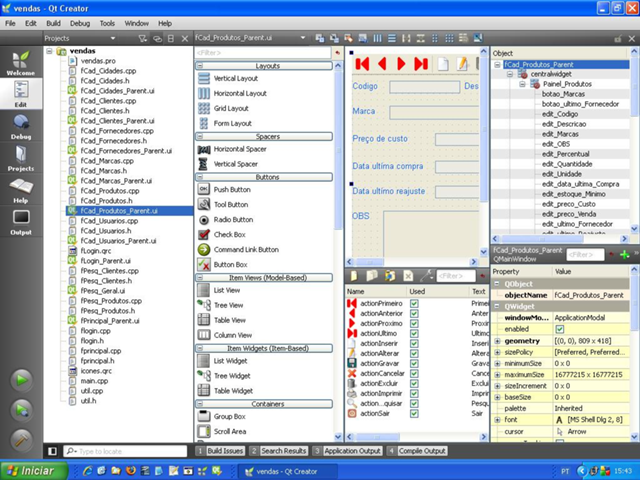
\includegraphics[width=1\textwidth]{./images/qtcreator.png}}
      \only<2>{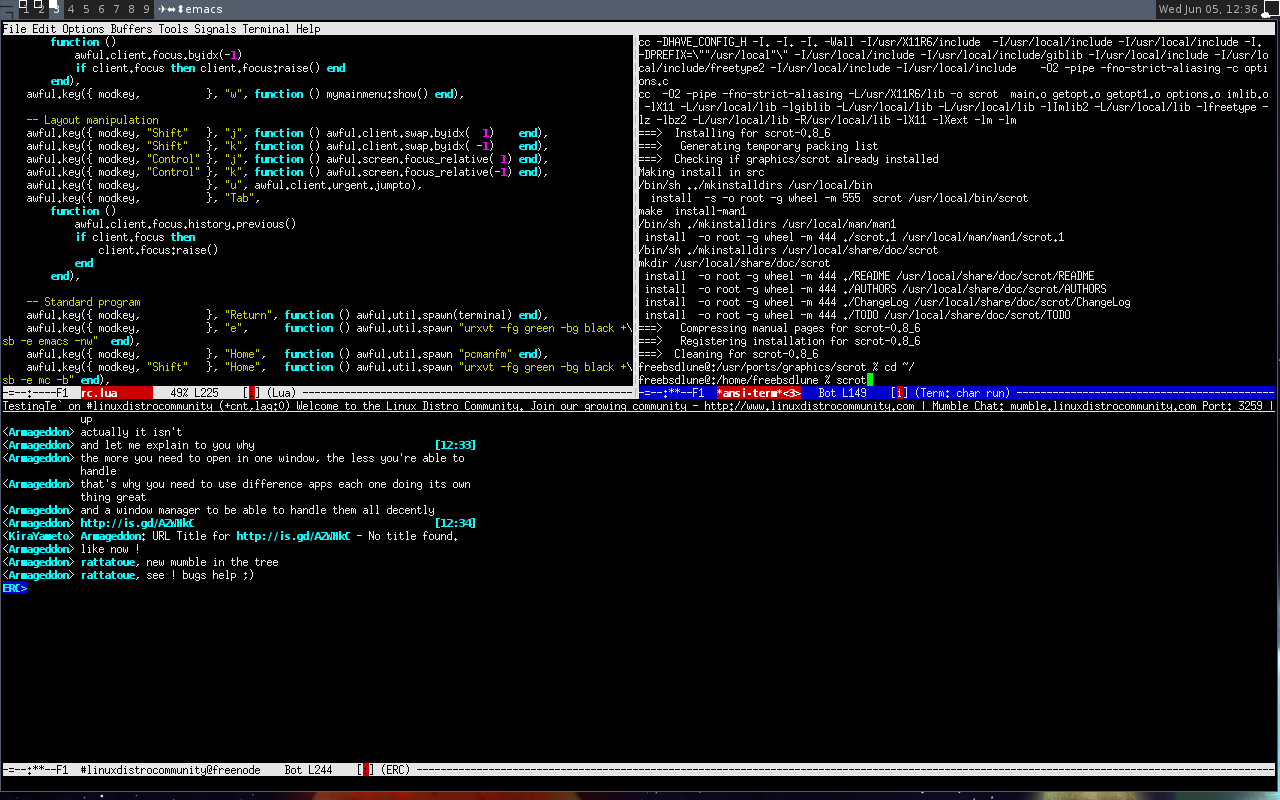
\includegraphics[width=1\textwidth]{./images/emacs.png}}}
  \end{figure}
\end{frame}

\begin{frame}
  \frametitle{Requirements}
  %\framesubtitle{Classification of SD-OCT volumes with LBP}
  \begin{block}{Spirit}\footnotesize
      \begin{itemize}
      \item The 2W: Will \& Wishes
      \end{itemize}
  \end{block}
  \begin{block}{Skill}\footnotesize
      \begin{itemize}
      \item Learn \& understand to parallelize on CPU and GPU
      \item Come back to the source - terminal/editor/compiler
      \item Move to linux
      \end{itemize}
  \end{block}
\end{frame}

\section{And the Future}

\begin{frame}
  \frametitle{And the Future}
  \begin{block}{Hardware}\footnotesize
      \begin{itemize}
      \item A new server 24 cores Intel Xeon 2700 and 128 GB + Tesla K40
      \item ODROID XU4: 2k screen capable + Octa Core $\rightarrow$ 74\$
      \item Investing money in Ultra-laptop or in the CCUB?
      \end{itemize}
      $\rightarrow$ Invest money in the cluster + odroid + laptop (or ubuntu phone)
  \end{block}
  \begin{figure}
    \centering{
      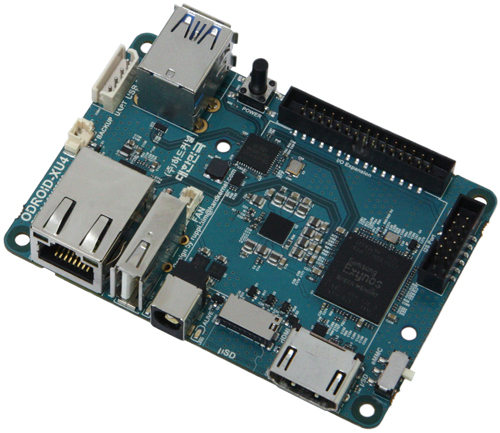
\includegraphics[width=.3\textwidth]{./images/odroid.jpg}}
  \end{figure}
\end{frame}

\end{document}